\everymath{\displaystyle}
\documentclass{beamer}
% \documentclass[handout]{beamer}

%\usepackage[pdftex]{color,graphicx}
\usepackage{amsmath,amssymb,amsfonts}

\mode<presentation>
{
  % \usetheme{Darmstadt}
  % \usetheme[hideothersubsections]{Hannover}
  % \usetheme[hideothersubsections]{Goettingen}
  \usetheme[hideothersubsections, right]{Berkeley}

  \usecolortheme{seahorse}
  % \usecolortheme{dolphin}
  \usecolortheme{rose}
  % \usecolortheme{orchid}

  \useinnertheme[shadow]{rounded}

  \setbeamercovered{transparent}
  % or whatever (possibly just delete it)
}

\mode<handout>{
  \setbeamercolor{background canvas}{bg=black!5}
  \usepackage{pgfpages}
  \pgfpagesuselayout{4 on 1}[a4paper,border shrink=5mm, landscape]
}

\usepackage[brazilian]{babel}
% or whatever

% \usepackage[latin1]{inputenc}
\usepackage[utf8]{inputenc}
% or whatever

\usepackage{times}
%\usepackage[T1]{fontenc}
% Or whatever. Note that the encoding and the font should match. If T1
% does not look nice, try deleting the line with the fontenc.


\title%[] % (optional, use only with long paper titles)
{Referências}

\subtitle
{Citações, Referências e Plágio} % (optional)

\author%[] % (optional, use only with lots of authors)
{Felipe Figueiredo}% \and S.~Another\inst{2}}
% - Use the \inst{?} command only if the authors have different
%   affiliation.

\institute[INTO] % (optional, but mostly needed)
{Instituto Nacional de Traumatologia e Ortopedia
}
  % \inst{1}%
  % Department of Computer Science\\
  % University of Somewhere
  % \and
  % \inst{2}%
  % Department of Theoretical Philosophy\\
  % University of Elsewhere}
% - Use the \inst command only if there are several affiliations.
% - Keep it simple, no one is interested in your street address.

\date%[] % (optional)
{}

% \subject{Talks}
% This is only inserted into the PDF information catalog. Can be left
% out.



% If you have a file called "university-logo-filename.xxx", where xxx
% is a graphic format that can be processed by latex or pdflatex,
% resp., then you can add a logo as follows:

\pgfdeclareimage[height=1.6cm]{university-logo}{../logo}
\logo{\pgfuseimage{university-logo}}



% Delete this, if you do not want the table of contents to pop up at
% the beginning of each subsection:
\AtBeginSubsection[]
%\AtBeginSection[]
{
  \begin{frame}<beamer>{Sumário}
    \tableofcontents[currentsection,currentsubsection]
  \end{frame}
}


% If you wish to uncover everything in a step-wise fashion, uncomment
% the following command:

% \beamerdefaultoverlayspecification{<+->}


\begin{document}

\begin{frame}
  \titlepage
\end{frame}

\begin{frame}{Sumário}
  \tableofcontents
  % You might wish to add the option [pausesections]
\end{frame}


%% Template
% \section{}

% \subsection{}

% \begin{frame}{}
%   \begin{itemize}
%   \item 
%   \end{itemize}
% \end{frame}

% \begin{frame}
%   \begin{columns}
%     \begin{column}{5cm}
%     \end{column}
%     \begin{column}{5cm}
%     \end{column}
%   \end{columns}
% \end{frame}

% \begin{frame}{}
%   \includegraphics[height=0.4\textheight]{file1}
%   \includegraphics[height=0.4\textheight]{file2}
%   \includegraphics[height=0.4\textheight]{file3}
%   \begin{figure}
%     \caption{}
%   \end{figure}
% \end{frame}

% \begin{frame}{}
%   \begin{definition}
%   \end{definition}
%   \begin{example}
%   \end{example}
%   \begin{block}{Exercício}
%   \end{block}
% \end{frame}


\section{Citações}

\begin{frame}{Citações}
  \begin{definition}[De acordo com a ABNT\ldots]
    Uma citação é a menção de uma informação extraída de outra fonte.
  \end{definition}
  \begin{example}[Fontes primárias]
    Livros, periódicos, teses, dissertações\ldots
  \end{example}
\end{frame}

\subsection{Citações Indiretas}

\begin{frame}{Citações Indiretas}
  \begin{definition}[Citação indireta]
    Uma citação indireta é a transcrição das informações ou dados da
    fonte original, com as palavras do autor (parafraseando).
  \end{definition}
  \begin{itemize}
  \item Estilo de citação mais usado em produções científicas
  \item Utilizada para citar informações, conclusões ou dados
  \item Formatos comuns de citação incluem: ``autor-ano'' e
    ``numérica''
  \end{itemize}
\end{frame}

\begin{frame}{Citações Indiretas}
  \begin{itemize}
  \item \alert{Toda} informação ou dado obtido da pesquisa
    bibliográfica \alert{deve} ter a fonte primária citada.
  \item Os autores e ano da fonte devem ser claramente especificados
  \item O autor do projeto \alert{não pode} reproduzir as palavras
    usadas (apenas as idéias ou informações)
  \end{itemize}
\end{frame}

\begin{frame}{Citações Indiretas}
  \begin{example}[Citação comum]
    Estudos anteriores \alert{(SILVA, J. et al, 2000)} indicam
    que\ldots
  \end{example}
  \begin{example}[Citação no texto]
    O grupo de José da Silva \alert{(2000)} observou que\ldots
  \end{example}
  \begin{example}[Citação numérica]
    Estudos anteriores \alert{(42)} indicam que que\ldots
  \end{example}
\end{frame}

\subsection{Citações Diretas}

\begin{frame}{Citações diretas}
  \begin{itemize}
  \item Utilizado para reproduzir fielmente as palavras usadas na
    fonte ({\em verbatim})
  \item Se curta ($\leq$ 3 linhas), usar aspas.
  \item Se longa ($>$ 3 linhas) deve ser destacado com:
    \begin{itemize}
    \item recuo da margem esquerda
    \item alinhado à direita
    \item espaçamento simples e fonte menor
    \end{itemize}
  \end{itemize}
\end{frame}

\subsection{Outras considerações}

\begin{frame}{Outras considerações}
  \begin{itemize}
  \item Se a fonte tiver {\bf mais de} 3 autores, usar o primeiro nome
    e a expressão \alert{et al} ({\em e outros}).
  \item Se a fonte não estiver disponível, pode ser feita a {\bf
      citação de citação}, com a expressão \alert{apud}
  \item Evitar o apud
  \end{itemize}
\end{frame}

\subsection{Aprofundamento}

\begin{frame}{Aprofundamento}
  \begin{block}{Leitura}
    Livro texto, seção {\bf 7.2}.
  \end{block}
\end{frame}

\section{Referências}

\subsection{Referências}

\begin{frame}{Referências}
  \begin{itemize}
  \item Devem constar em capítulo à parte (após a Conclusão, antes dos
    Apêndices)
  \item Detalham as informações bibliográficas de cada fonte citada
  \item Formatação padronizada das fontes
  \item Formato específico para cada tipo de fonte (artigo, livro,
    capítulo de livro, tese, etc)
  \end{itemize}
\end{frame}
\subsection{Formatos comuns}

\begin{frame}{Formato ABNT}
  Principais aspectos
  \begin{itemize}
  \item Autor (sobrenome) em caixa alta, iniciais dos nomes;
  \item Referências: ordem alfabética do primeiro autor;
  \item Título em itálico, Publicação em negrito;
  \item Citação: AUTOR, ano.
  \end{itemize}
  \begin{example}[Citação]
    O grupo de José Silva (SILVA, J. et al, 2000) observou que\ldots
  \end{example}
  \begin{example}[Referência]
    SILVA, J., et al {\em Título do artigo}, {\bf Revista Qualis A},
    2000.
  \end{example}
\end{frame}

\begin{frame}{Formato Vancouver}
  \begin{itemize}
  \item Autor: sobrenome e iniciais dos nomes;
  \item Referências: ordem de citação;
  \item Citação: numérica, em parênteses ou colchetes.
  \end{itemize}
  \begin{example}[Citação]
    O grupo de José Silva [42] observou que\ldots
  \end{example}
  \begin{example}[Referência]
    42. Silva, J., et al. Título do artigo, Revista Qualis A, 2000.
  \end{example}
\end{frame}

\subsection{Aprofundamento}

\begin{frame}{Aprofundamento}
  \begin{block}{Leitura}
    Livro texto, seções {\bf 7.1} e {\bf 7.3}.
  \end{block}
\end{frame}

\subsection{Gerenciadores de Referências}

\begin{frame}{Gerenciadores pessoais de referências}
  \begin{itemize}
  \item Antigamente se organizavam as referências a ser citadas com
    fichas bibliográficas (fichamento)
  \item Agora, estamos no século XXI.
  \item Softwares especializados facilitam o trabalho de organização
    (e citação!) das referências estudadas
  \item Alguns exemplos de bases de referências muito utilizados:
    \begin{itemize}
    \item<4-> \alert<5->{Mendeley}
    \item<4-> EndNote
    \item<4-> Zotero
    \item<4-> Roundcube
    \end{itemize}
  \end{itemize}
\end{frame}

\begin{frame}{Gerenciadores pessoais de referências}
  Esses softwares oferecem (entre outras coisas):
  \begin{itemize}
  \item Importação de metadados da internet
  \item Importação de referências de outros softwares
  \item Plugin do Word para
    \begin{itemize}
    \item<3-> citações
    \item<3-> bibliografia
    \end{itemize}
  \item Formatação de citações e bibliografia
  \item Rede social (compartilhar referências entre colegas)
  \end{itemize}
\end{frame}

\subsection{Mendeley}

\begin{frame}{Mendeley (menu)}
  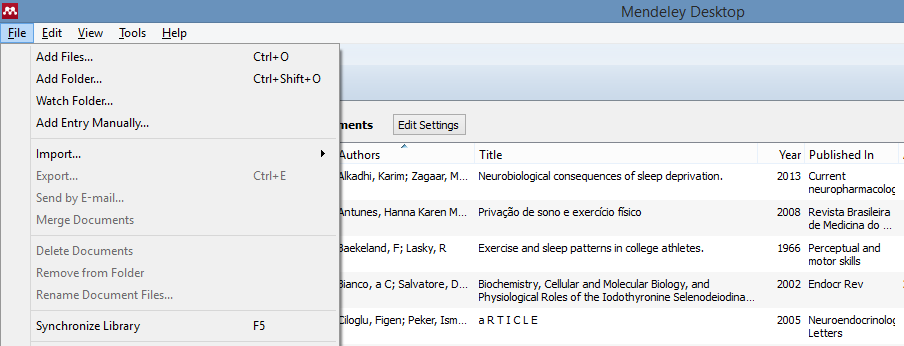
\includegraphics[width=1.2\textwidth]{Referencias/mendeley-menu}
\end{frame}

\begin{frame}{Mendeley (visão artigo)}
  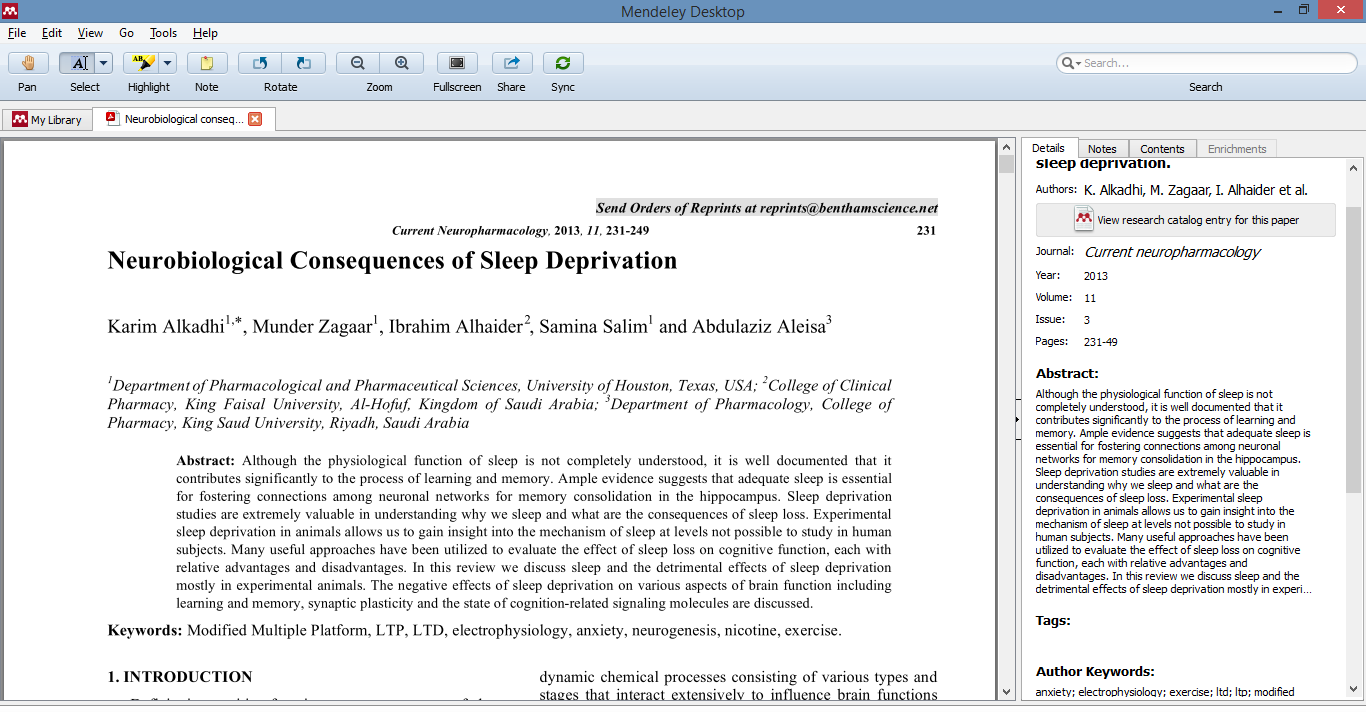
\includegraphics[width=1.2\textwidth]{Referencias/mendeley-artigo}
\end{frame}

\begin{frame}{Metadados no Mendeley}
  \begin{itemize}
  \item Metadados incompletos podem ser preenchidos automaticamente
  \item Por vezes, o título (completo) é suficiente
  \item Se disponível, use o DOI do artigo para buscar os metadados
  \item O DOI do artigo pode ser obtido no CrossRef
    \footnote{http://www.crossref.org/}
  \end{itemize}
\end{frame}

\begin{frame}{Metadados no Mendeley}
  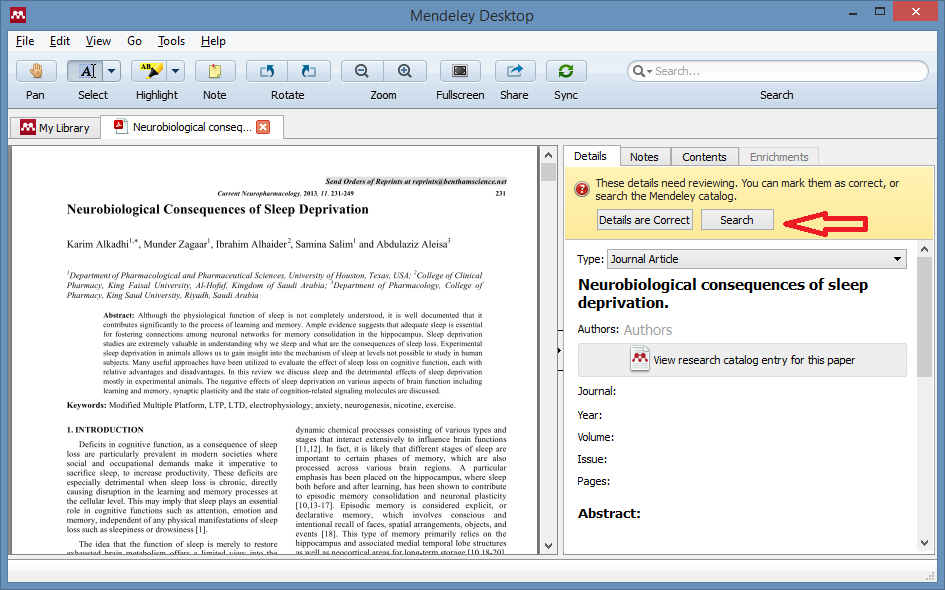
\includegraphics[width=\textwidth]{Referencias/mendeley-busca1}
\end{frame}

\begin{frame}{Metadados no Mendeley}
  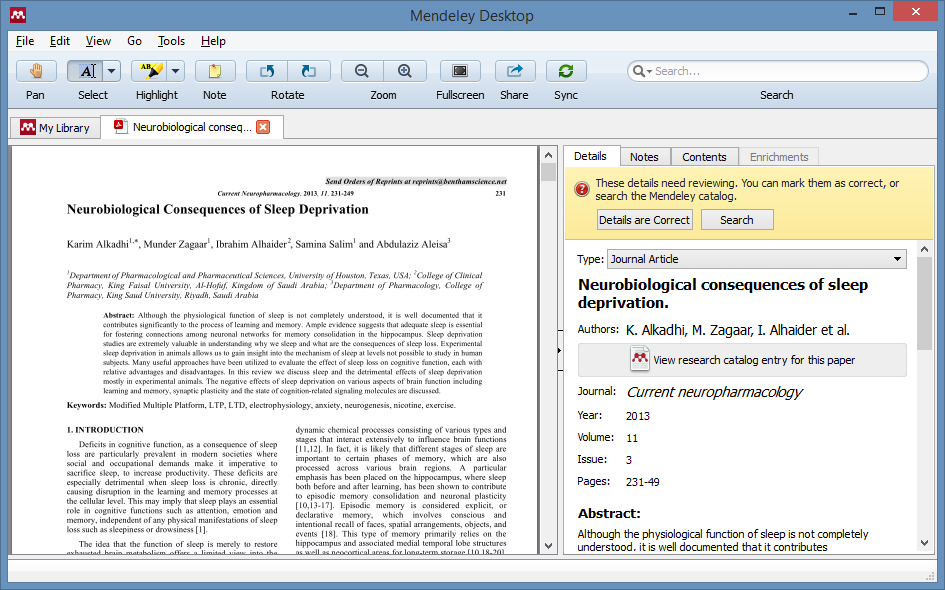
\includegraphics[width=\textwidth]{Referencias/mendeley-busca2}
\end{frame}

\begin{frame}{Mendeley no Word}
  \begin{itemize}
  \item No Mendeley, instale o {\em plugin} do Word
  \item Na aba {\em Referências} use a opção \alert{Insert Citation}
    do Mendeley para citar no texto corrente
  \item Escolha um estilo de formatação de citações e referências
  \item No capítulo {\bf Bibliografia} use a opção do Mendeley
    \alert{Insert Bibliography}
  \end{itemize}
\end{frame}

\begin{frame}{Mendeley no Word}
  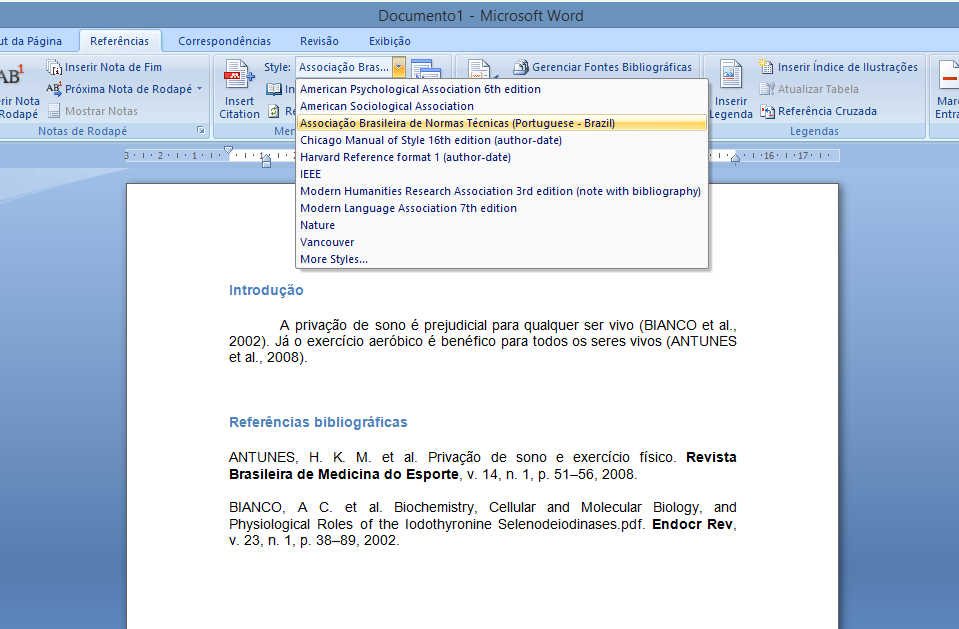
\includegraphics[width=1.1\textwidth]{Referencias/mendeley-word-ABNT}
\end{frame}

\begin{frame}{Mendeley no Word}
  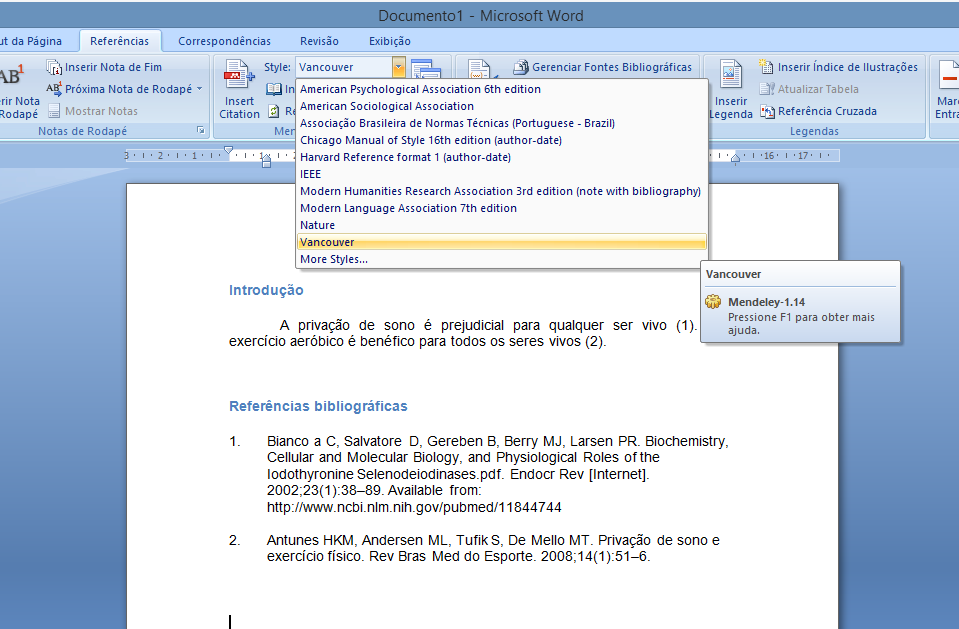
\includegraphics[width=1.1\textwidth]{Referencias/mendeley-word-vancouver}
\end{frame}

\begin{frame}{Dicas para usar o Mendeley}
  \begin{itemize}
  \item Manter \alert{todos} os PDFs dos papers em um diretório
    ``central'', organizando temas em sub-diretórios
  \item Faça o Mendeley \alert{monitorar} essa ``pasta central'' ({\em
      File/Watch folder})
  \item Confira se a importação dos metadados foi correta e completa
  \item Se quiser corrigir os metadados, arraste a referência para a
    seção {\em Needs review} para ativar a opção {\em Search}.
  \item Digite manualmente apenas as referências que não puderem ser
    obtidas automaticamente (provavelmente poucas)
  \end{itemize}
\end{frame}

\section{Plágio}

\subsection{Plágio}

\begin{frame}{Plágio}
  \begin{definition}
    O plágio acadêmico se configura quando um aluno retira, seja de
    livros ou da Internet, ideias, conceitos ou frases de outro autor
    (que as formulou e as publicou), sem lhe dar o devido crédito, sem
    citá-lo como fonte de pesquisa.
  \end{definition}

  Fonte: Cartilha UFF
\end{frame}

\begin{frame}{Tipos de plágio}
  \begin{definition}[Plágio integral]
    O autor \alert{reproduz} o texto da fonte, sem citá-la.
  \end{definition}
  \begin{definition}[Plágio parcial]
    \begin{itemize}
    \item Modificar trechos ou palavras da fonte, sem citar a fonte
    \item Fazer uma colagem de trechos de várias fontes (mosaico), sem
      citar \alert{todas} as fontes
    \item \alert{Mesmo citando}, modificar palavras, mas não destacar
      o texto entre aspas (citação direta!)
    \end{itemize}
  \end{definition}
  \begin{definition}[Plágio conceitual]
    O autor altera substancialmente o texto, parafraseando, mas não
    cita a fonte
  \end{definition}
\end{frame}

\subsection{Detecção automática}

\begin{frame}{Detecção automática de plágio}
  \begin{itemize}
  \item Mecanismos de busca (Google, Yahoo, etc) localizam trechos de
    texto mesmo com substituições e omissões
  \item Softwares especialistas automatizam esse processo
  \end{itemize}
\end{frame}

\begin{frame}{CopySpider}
  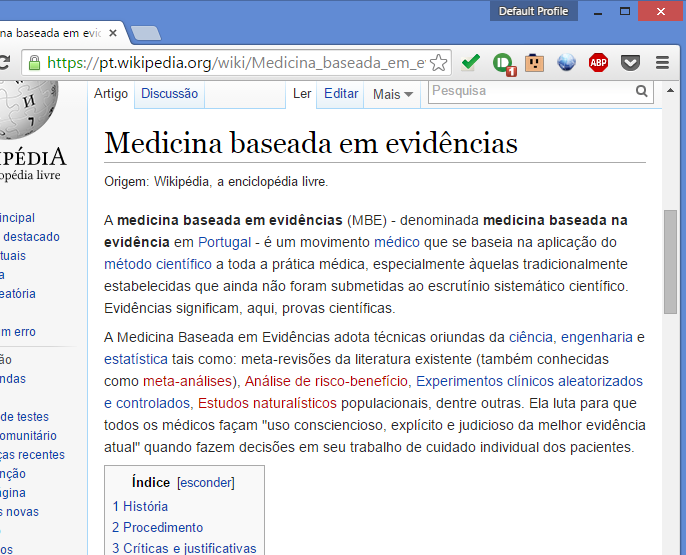
\includegraphics[height=.95\textheight]{Referencias/fonte}
\end{frame}

\begin{frame}{CopySpider}
  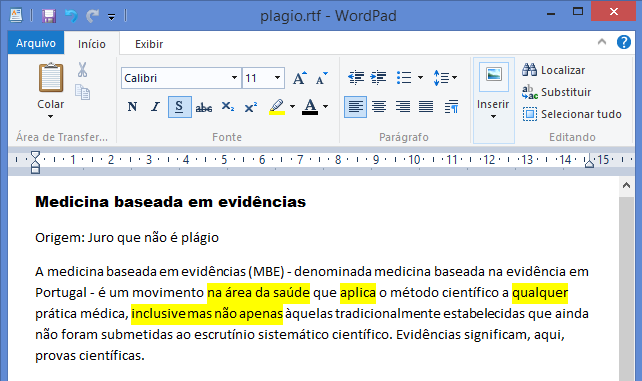
\includegraphics[width=\textwidth]{Referencias/plagio}
\end{frame}

\begin{frame}{CopySpider}
  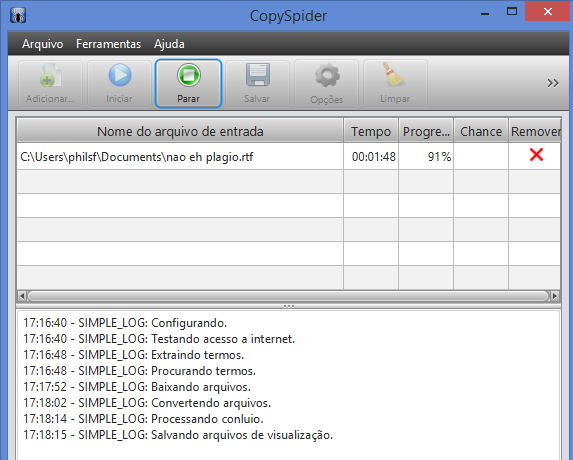
\includegraphics[height=.95\textheight]{Referencias/copyspider1}
\end{frame}

\begin{frame}{CopySpider}
  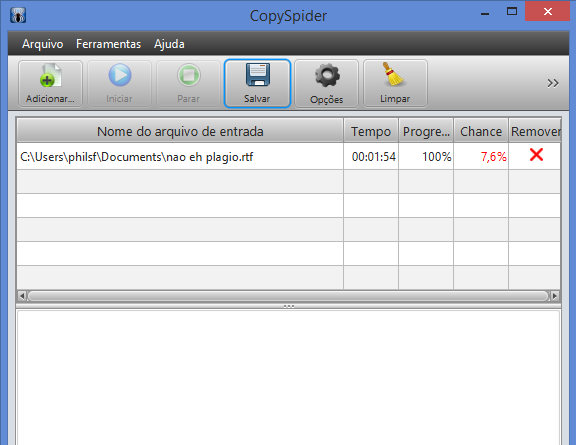
\includegraphics[height=.95\textheight]{Referencias/copyspider2}
\end{frame}

\begin{frame}{CopySpider}
  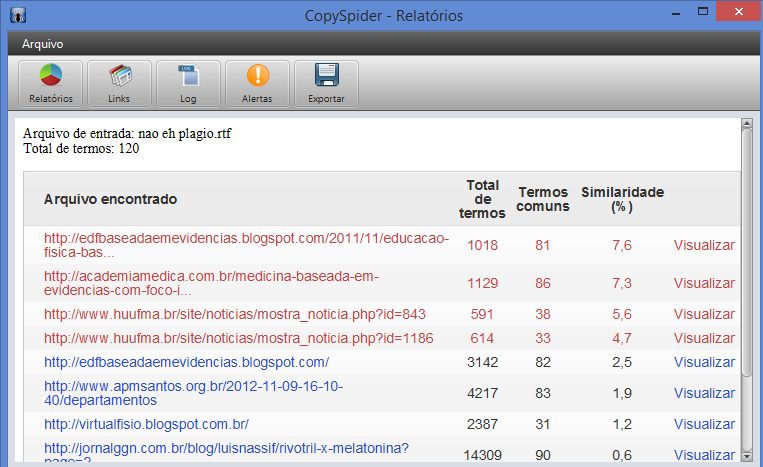
\includegraphics[width=\textwidth]{Referencias/copyspider3}
\end{frame}

\begin{frame}{CopySpider}
  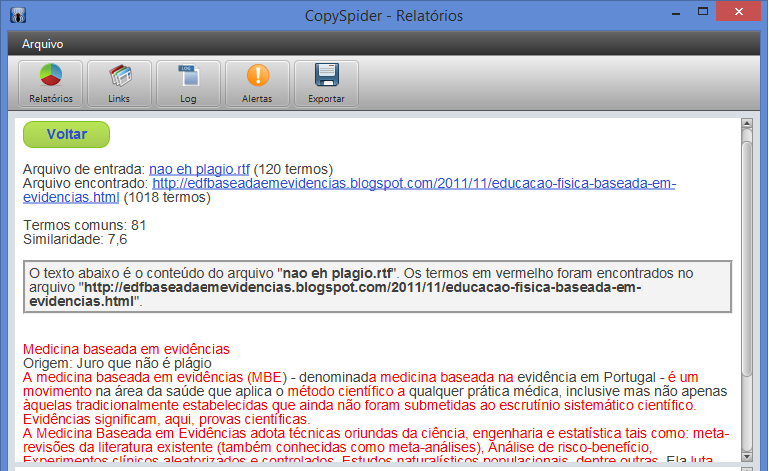
\includegraphics[width=\textwidth]{Referencias/copyspider4}
\end{frame}

\section{Referências}

\subsection{Referências}

\begin{frame}{Referências}
  \begin{itemize}
  \item<1-> Mendeley: \url{http://www.mendeley.com}
  \item<1-> Cartilha UFF: \url{http://www.noticias.uff.br/arquivos/cartilha-sobre-plagio-academico.pdf}
  \end{itemize}
\end{frame}

\end{document}
